\documentclass[tikz,border=3pt]{standalone}
\usepackage{fontspec}
\IfFontExistsTF{Times New Roman}
  {\setmainfont{Times New Roman}}
  {\setmainfont{TeX Gyre Termes}}
\usepackage{amsmath,amssymb}
\usepackage{xcolor}
\usepackage{tikz}
\usetikzlibrary{arrows.meta,positioning,calc,fit,backgrounds,shapes.geometric,decorations.pathreplacing,pgfplots.groupplots}
\definecolor{QFlowNavy}{HTML}{17365D}
\definecolor{QFlowBlue}{HTML}{2F5597}
\definecolor{QFlowTeal}{HTML}{2A7F7F}
\definecolor{QFlowAmber}{HTML}{8B5A00}
\definecolor{QFlowGray}{HTML}{667085}
\definecolor{QFlowLine}{HTML}{CBD5E1}
\definecolor{QFlowPaleBlue}{HTML}{EAF1F8}
\definecolor{QFlowPaleGray}{HTML}{F2F4F7}
\tikzset{
  qbox/.style={draw=QFlowNavy,rounded corners=1.2mm,fill=white,
    line width=0.6pt,align=center,inner sep=2.2mm,font=\fontsize{8.5}{10}\selectfont},
  qsoft/.style={qbox,fill=QFlowPaleBlue},
  qoutside/.style={qbox,draw=QFlowGray,dashed,fill=QFlowPaleGray},
  qarrow/.style={-{Latex[length=2mm,width=1.3mm]},line width=0.7pt,QFlowNavy},
  qdasharrow/.style={qarrow,dashed,QFlowGray},
  qlabel/.style={font=\fontsize{8}{9.2}\selectfont,align=center},
  qsmall/.style={font=\fontsize{7.5}{8.7}\selectfont,align=center}
}

\begin{document}
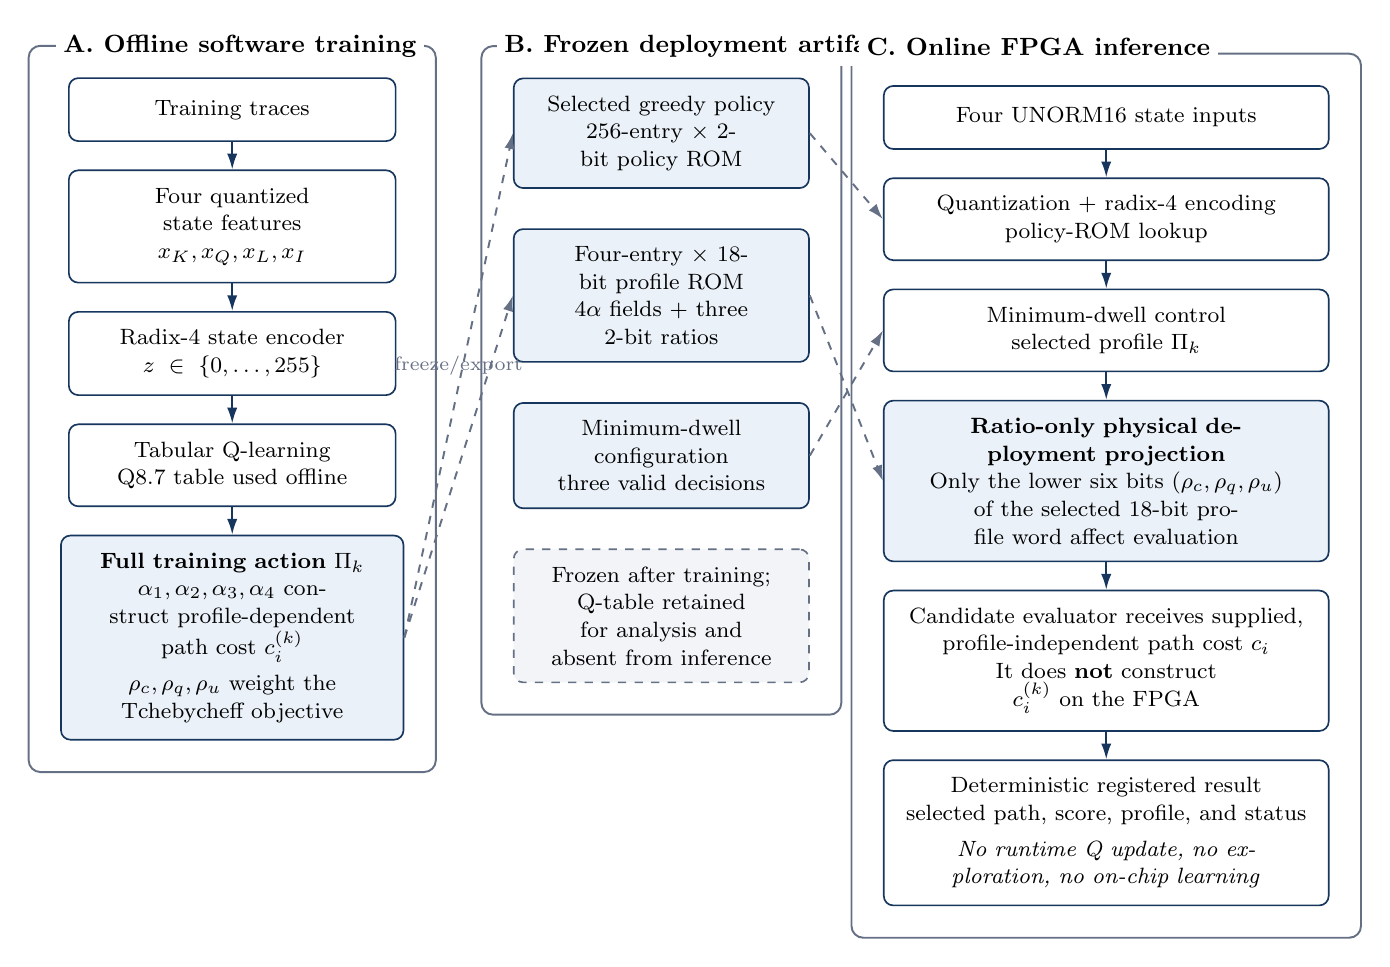
\begin{tikzpicture}[x=1cm,y=1cm]
  \tikzset{
    region/.style={draw=QFlowGray,rounded corners=1.5mm,line width=0.7pt},
    trainstep/.style={qbox,minimum width=4.15cm,text width=3.65cm,minimum height=8mm},
    artifact/.style={qsoft,minimum width=3.75cm,text width=3.25cm,minimum height=9mm},
    online/.style={qbox,minimum width=5.65cm,text width=5.1cm,minimum height=8mm}
  }

  \node[qlabel,anchor=west,fill=white,inner sep=1mm,font=\fontsize{9}{10.5}\selectfont\bfseries] at (0.05,0.65)
    {A. Offline software training};
  \node[qlabel,anchor=west,fill=white,inner sep=1mm,font=\fontsize{9}{10.5}\selectfont\bfseries] at (5.65,0.65)
    {B. Frozen deployment artifacts};
  \node[qlabel,anchor=west,fill=white,inner sep=1mm,font=\fontsize{9}{10.5}\selectfont\bfseries] at (10.25,0.65)
    {C. Online FPGA inference};

  \node[trainstep] (traces) at (2.3,-0.15) {Training traces};
  \node[trainstep,below=3.5mm of traces] (features) {Four quantized state features\\$x_K,x_Q,x_L,x_I$};
  \node[trainstep,below=3.5mm of features] (encoder) {Radix-4 state encoder\\$z\in\{0,\ldots,255\}$};
  \node[trainstep,below=3.5mm of encoder] (qlearn) {Tabular Q-learning\\Q8.7 table used offline};
  \node[qsoft,minimum width=4.35cm,text width=3.85cm,below=3.5mm of qlearn] (full)
    {\textbf{Full training action $\Pi_k$}\\
    $\alpha_1,\alpha_2,\alpha_3,\alpha_4$ construct profile-dependent path cost $c_i^{(k)}$\\[1mm]
    $\rho_c,\rho_q,\rho_u$ weight the Tchebycheff objective};
  \draw[qarrow] (traces)--(features);
  \draw[qarrow] (features)--(encoder);
  \draw[qarrow] (encoder)--(qlearn);
  \draw[qarrow] (qlearn)--(full);

  \node[artifact] (policy) at (7.75,-0.45) {Selected greedy policy\\256-entry $\times$ 2-bit policy ROM};
  \node[artifact,below=5mm of policy] (profiles) {Four-entry $\times$ 18-bit profile ROM\\$4\alpha$ fields + three 2-bit ratios};
  \node[artifact,below=5mm of profiles] (dwellcfg) {Minimum-dwell configuration\\three valid decisions};
  \node[qoutside,minimum width=3.75cm,text width=3.25cm,below=5mm of dwellcfg] (frozen)
    {Frozen after training; Q-table retained for analysis and absent from inference};
  \draw[qdasharrow] (full.east) -- node[qsmall,above]{freeze/export} (policy.west);
  \draw[qdasharrow] (full.east) -- (profiles.west);

  \node[online] (statein) at (13.4,-0.25) {Four UNORM16 state inputs};
  \node[online,below=3.5mm of statein] (lookup) {Quantization + radix-4 encoding\\policy-ROM lookup};
  \node[online,below=3.5mm of lookup] (dwell) {Minimum-dwell control\\selected profile $\Pi_k$};
  \node[qsoft,minimum width=5.65cm,text width=5.1cm,below=3.5mm of dwell] (projection)
    {\textbf{Ratio-only physical deployment projection}\\Only the lower six bits $(\rho_c,\rho_q,\rho_u)$ of the selected 18-bit profile word affect evaluation};
  \node[online,below=3.5mm of projection] (eval)
    {Candidate evaluator receives supplied, profile-independent path cost $c_i$\\It does \textbf{not} construct $c_i^{(k)}$ on the FPGA};
  \node[online,below=3.5mm of eval] (out)
    {Deterministic registered result\\selected path, score, profile, and status\\[1mm]
    \textit{No runtime Q update, no exploration, no on-chip learning}};
  \draw[qarrow] (statein)--(lookup);
  \draw[qarrow] (lookup)--(dwell);
  \draw[qarrow] (dwell)--(projection);
  \draw[qarrow] (projection)--(eval);
  \draw[qarrow] (eval)--(out);
  \draw[qdasharrow] (policy.east) -- (lookup.west);
  \draw[qdasharrow] (profiles.east) -- (projection.west);
  \draw[qdasharrow] (dwellcfg.east) -- (dwell.west);

  \begin{scope}[on background layer]
    \node[region,fit=(traces)(full),inner sep=4mm] {};
    \node[region,fit=(policy)(frozen),inner sep=4mm] {};
    \node[region,fit=(statein)(out),inner sep=4mm] {};
  \end{scope}
\end{tikzpicture}
\end{document}
